% !Mode:: "TeX:UTF-8"
% \textbf{类比探究专练之旋转结构(一)}
% T22(题号)-A(难度ABC)03(序号)

\begin{defproblem}{T22-A01-01}%
\begin{onlyproblem}%
如图1,$\angle QPN$的顶点$P$在正方形$ABCD$两条对角线交点处,$\angle QPN=\alpha $,将$\angle QPN$绕点$P$旋转,旋转过程中$\angle QPN$的两边分别与正方形$ABCD$的边$AD$和$CD$交于点$E$和点$F$(点$F$与点$C$,$D$不重合).

(1)如图1,当$\alpha =90^{\circ }$时,$DE$,$DF$,$AD$之间满足的数量关系是{\_}{\_}{\_}{\_}{\_}{\_}{\_}{\_}{\_}{\_}{\_}{\_}{\_}{\_}{\_};

(2)如图2,将图1中的正方形$ABCD$改为$\angle ADC=120^{\circ }$的菱形,其他条件不变,当$\alpha =60^{\circ }$时,(1)中的结论变为{\_}{\_}{\_}{\_}{\_}{\_}{\_}{\_}{\_}{\_}{\_}{\_}{\_}{\_},请给出证明;

(3)在(2)的条件下,若旋转过程中$\angle QPN$的边$PQ$与射线$AD$交于点$E$,其他条件不变,当点$E$落在线段$AD$的延长线上时,探究$DE$,$DF$,$AD$之间的数量关系(直接写出结论,不用加以证明).
\begin{center}
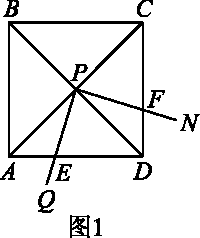
\includegraphics[scale=0.8]{T22-A01-01-01.pdf}\qquad
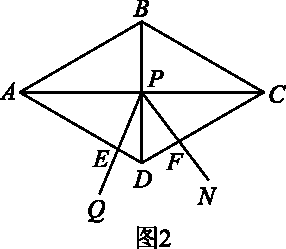
\includegraphics[scale=0.8]{T22-A01-01-02.pdf}\qquad
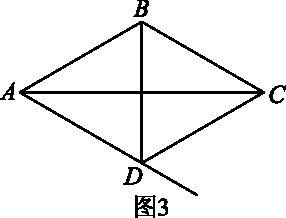
\includegraphics[scale=0.8]{T22-A01-01-03.pdf}
\end{center}
% \begin{flushright}
% 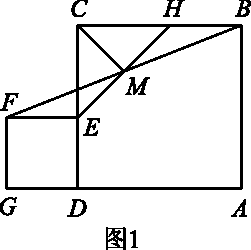
\includegraphics[scale=0.8]{T22-A03-01.pdf}\\
% 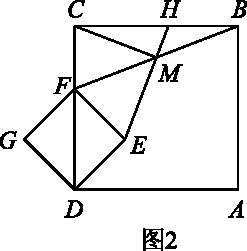
\includegraphics[scale=0.8]{T22-A03-02.pdf}\\
% 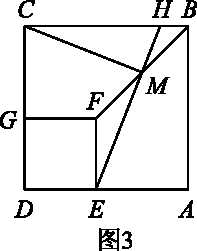
\includegraphics[scale=0.8]{T22-A03-03.pdf}
% \end{flushright}

\end{onlyproblem}%
\begin{onlysolution}%
\begin{center}
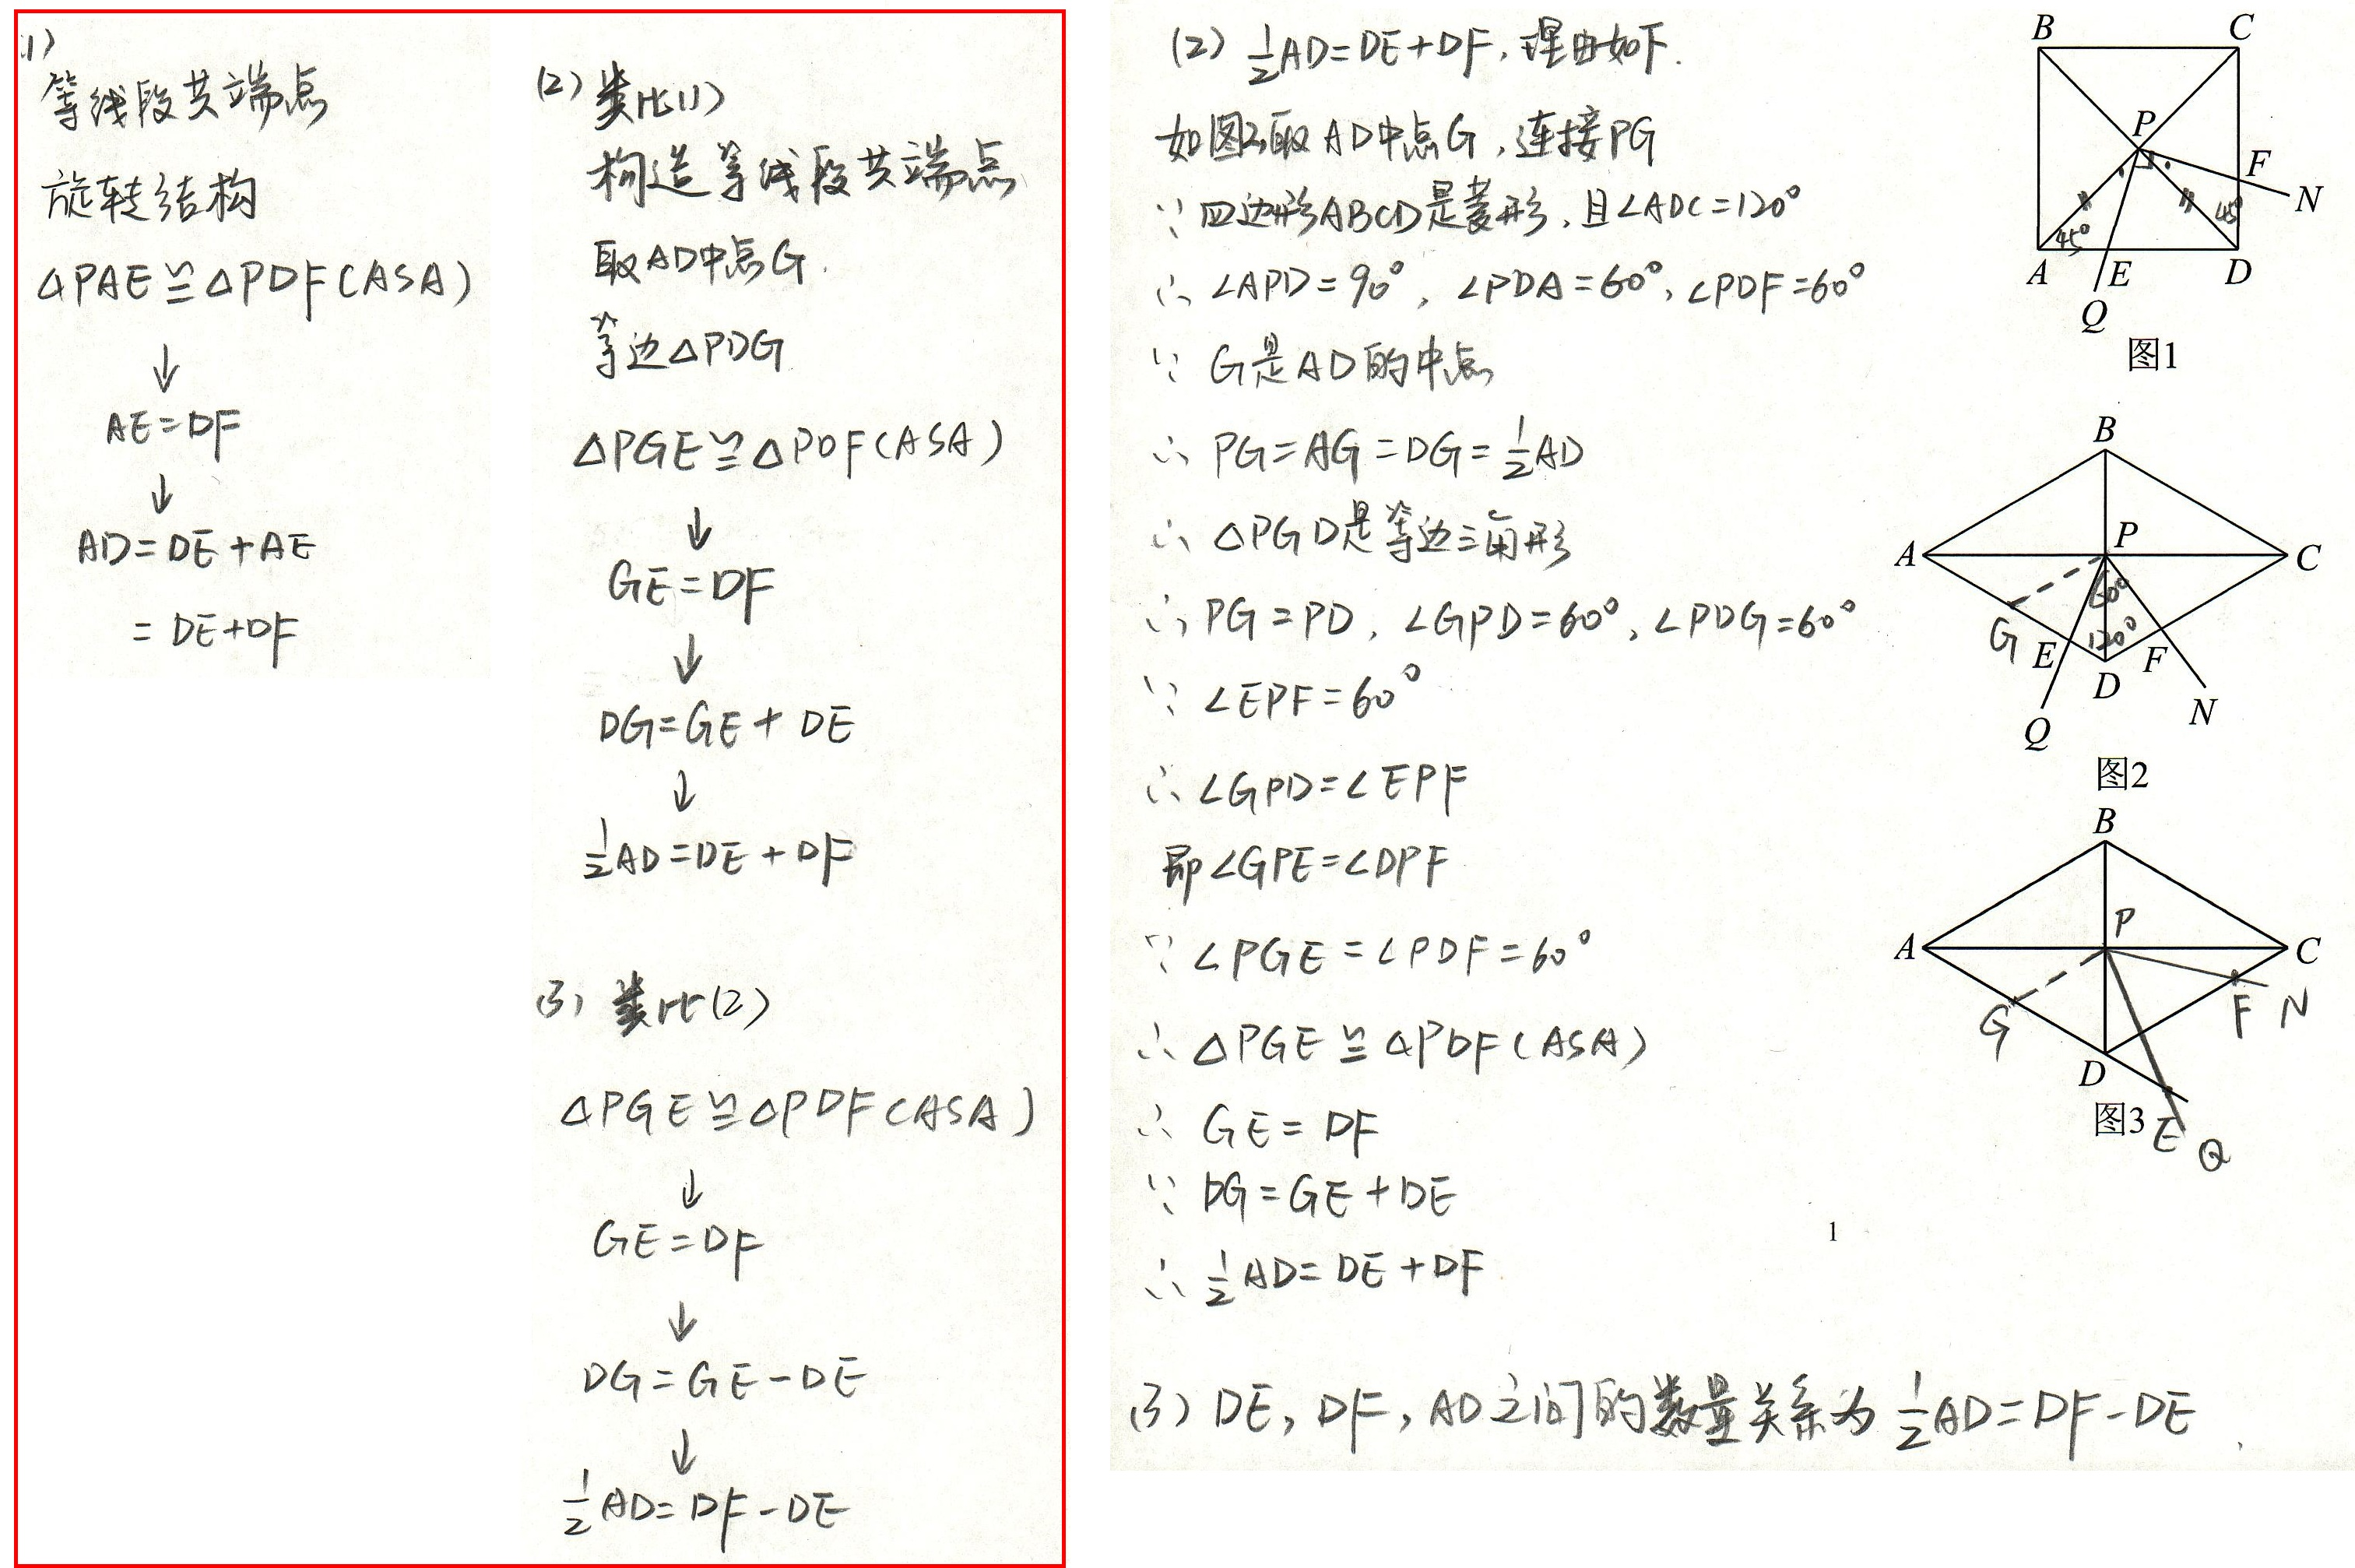
\includegraphics[width=.95\textwidth]{T22-A01-01-04-Ans.jpg}
\end{center}
\end{onlysolution}%
\end{defproblem}

\begin{defproblem}{T22-A01-02}%
\begin{onlyproblem}%
(2018--2019学年上学期九年级郑州期末10分)如图,$\triangle ABC$和$\triangle ADE$是有公共顶点的直角三角形,$\angle BAC=\angle DAE=90^{\circ }$,点$P$为射线$BD$,$CE$的交点.

(1)如图1,若$\triangle ABC$和$\triangle ADE$是等腰三角形,求证:$\angle ABD=\angle ACE$;

(2)如图2,若$\angle ADE=\angle ABC=30^{\circ }$,问:(1)中的结论是否成立?请说明理由.

(3)在(1)的条件下,$AB=6$,$AD=4$,若把$\triangle ADE$绕点$A$旋转,当$\angle EAC=90^{\circ }$时,请直接写出$PB$的长度.
\begin{center}
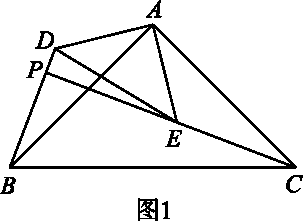
\includegraphics[scale=0.8]{T22-A01-02-01.pdf}\qquad
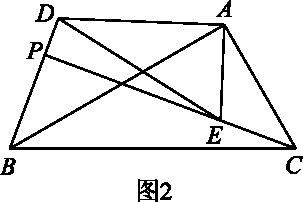
\includegraphics[scale=0.8]{T22-A01-02-02.pdf}\qquad
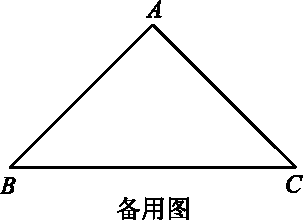
\includegraphics[scale=0.8]{T22-A01-02-03.pdf}
\end{center}
% \begin{flushright}
% 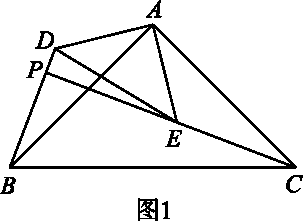
\includegraphics[scale=0.8]{T22-A01-02-01.pdf}\\
% 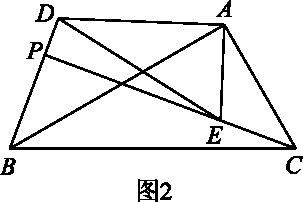
\includegraphics[scale=0.8]{T22-A01-02-02.pdf}\\
% 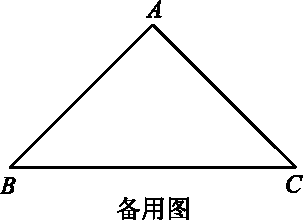
\includegraphics[scale=0.8]{T22-A01-02-03.pdf}
% \end{flushright}

\end{onlyproblem}%
\begin{onlysolution}%
\begin{center}
% \includegraphics[width=.95\textwidth]{T22-A01-02-04-Ans.jpg}
\end{center}
\end{onlysolution}%
\end{defproblem}


\begin{defproblem}{T22-A01-03}%
\begin{onlyproblem}%
(2017--2018学年上学期九年级郑州期末10分)如图,在Rt$ABC$中,$\angle ACB=90^{\circ }$,$\angle A=30^{\circ }$,点$O$为$AB$的中点,点$P$为直线$BC$上的动点(不与点$B$、点$C$重合),连接$OC$,$OP$,将线段$OP$绕点$P$顺时针旋转60$^{\circ }$,得到线段$PQ$,连接$BQ$.

(1)如图1,当点$P$在线段$BC$上时,请直接写出线段$BQ$与$CP$的数量关系:{\_}{\_}{\_}{\_}{\_}{\_}{\_}{\_}{\_}{\_};

(2)如图2,当点$P$在$CB$延长线上时,(1)中结论是否成立?若成立,请加以证明;若不成立,请说明理由;

(3)如图3,当点$P$在$BC$延长线上时,若$\angle BPO=15^{\circ }$,$BP=4$,请求出$BQ$的长.
\begin{center}
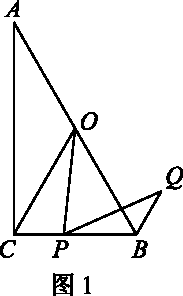
\includegraphics[scale=0.8]{T22-A01-03-01.pdf}\qquad
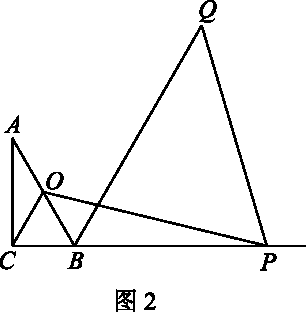
\includegraphics[scale=0.8]{T22-A01-03-02.pdf}\qquad
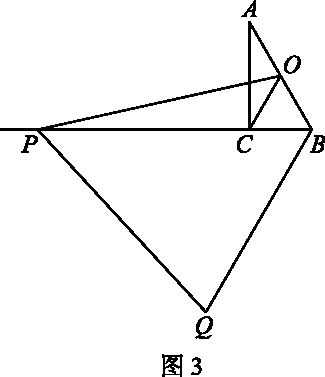
\includegraphics[scale=0.8]{T22-A01-03-03.pdf}
\end{center}
% \begin{flushright}
% 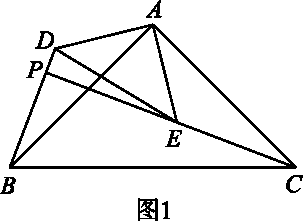
\includegraphics[scale=0.8]{T22-A01-02-01.pdf}\\
% 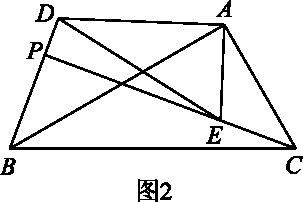
\includegraphics[scale=0.8]{T22-A01-02-02.pdf}\\
% 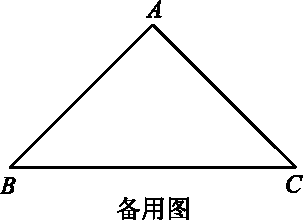
\includegraphics[scale=0.8]{T22-A01-02-03.pdf}
% \end{flushright}

\end{onlyproblem}%
\begin{onlysolution}%
\begin{center}
% \includegraphics[width=.95\textwidth]{T22-A01-02-04-Ans.jpg}
\end{center}
\end{onlysolution}%
\end{defproblem}


\begin{defproblem}{T22-A01-04}%
\begin{onlyproblem}%
已知,$\triangle ABC$为等边三角形,点$D$为直线$BC$上一动点(点$D$不与$B$,$C$重合).以$AD$为边作菱形$ADEF$,使$\angle DAF=60^{\circ }$,连接$CF$.

\textbf{初步感知}:(1)如图1,当点$D$在边$BC$上时,

①求证:$\angle ADB=\angle AFC$;

②请直接判断结论$\angle AFC=\angle ACB+\angle DAC$是否成立.

\textbf{问题探究}:(2)如图2,当点$D$在边$BC$的延长线上时,其他条件不变,结论$\angle AFC=\angle ACB+\angle DAC$是否成立?请写出$\angle AFC$,$\angle ACB$,$\angle DAC$之间存在的数量关系,并写出证明过程.

\textbf{类比分析}:(3)如图3,当点$D$在边$CB$的延长线上时,且点$A$,$F$分别在直线$BC$的异侧,其他条件不变,请补全图形,并直接写出$\angle AFC$,$\angle ACB$,$\angle DAC$之间存在的等量关系.
\begin{center}
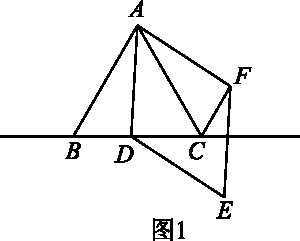
\includegraphics[scale=0.8]{T22-A01-04-01.pdf}\qquad
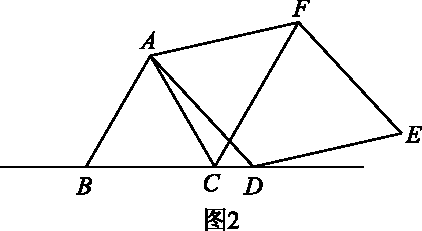
\includegraphics[scale=0.8]{T22-A01-04-02.pdf}\qquad
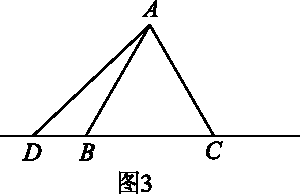
\includegraphics[scale=0.8]{T22-A01-04-03.pdf}
\end{center}
% \begin{flushright}
% 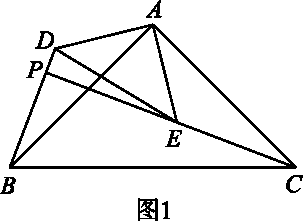
\includegraphics[scale=0.8]{T22-A01-02-01.pdf}\\
% 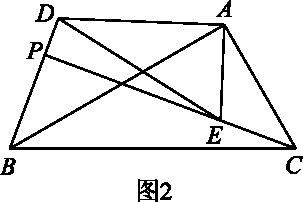
\includegraphics[scale=0.8]{T22-A01-02-02.pdf}\\
% 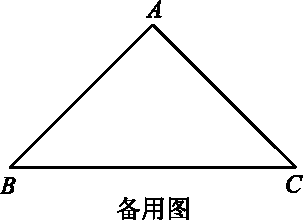
\includegraphics[scale=0.8]{T22-A01-02-03.pdf}
% \end{flushright}

\end{onlyproblem}%
\begin{onlysolution}%
\begin{center}
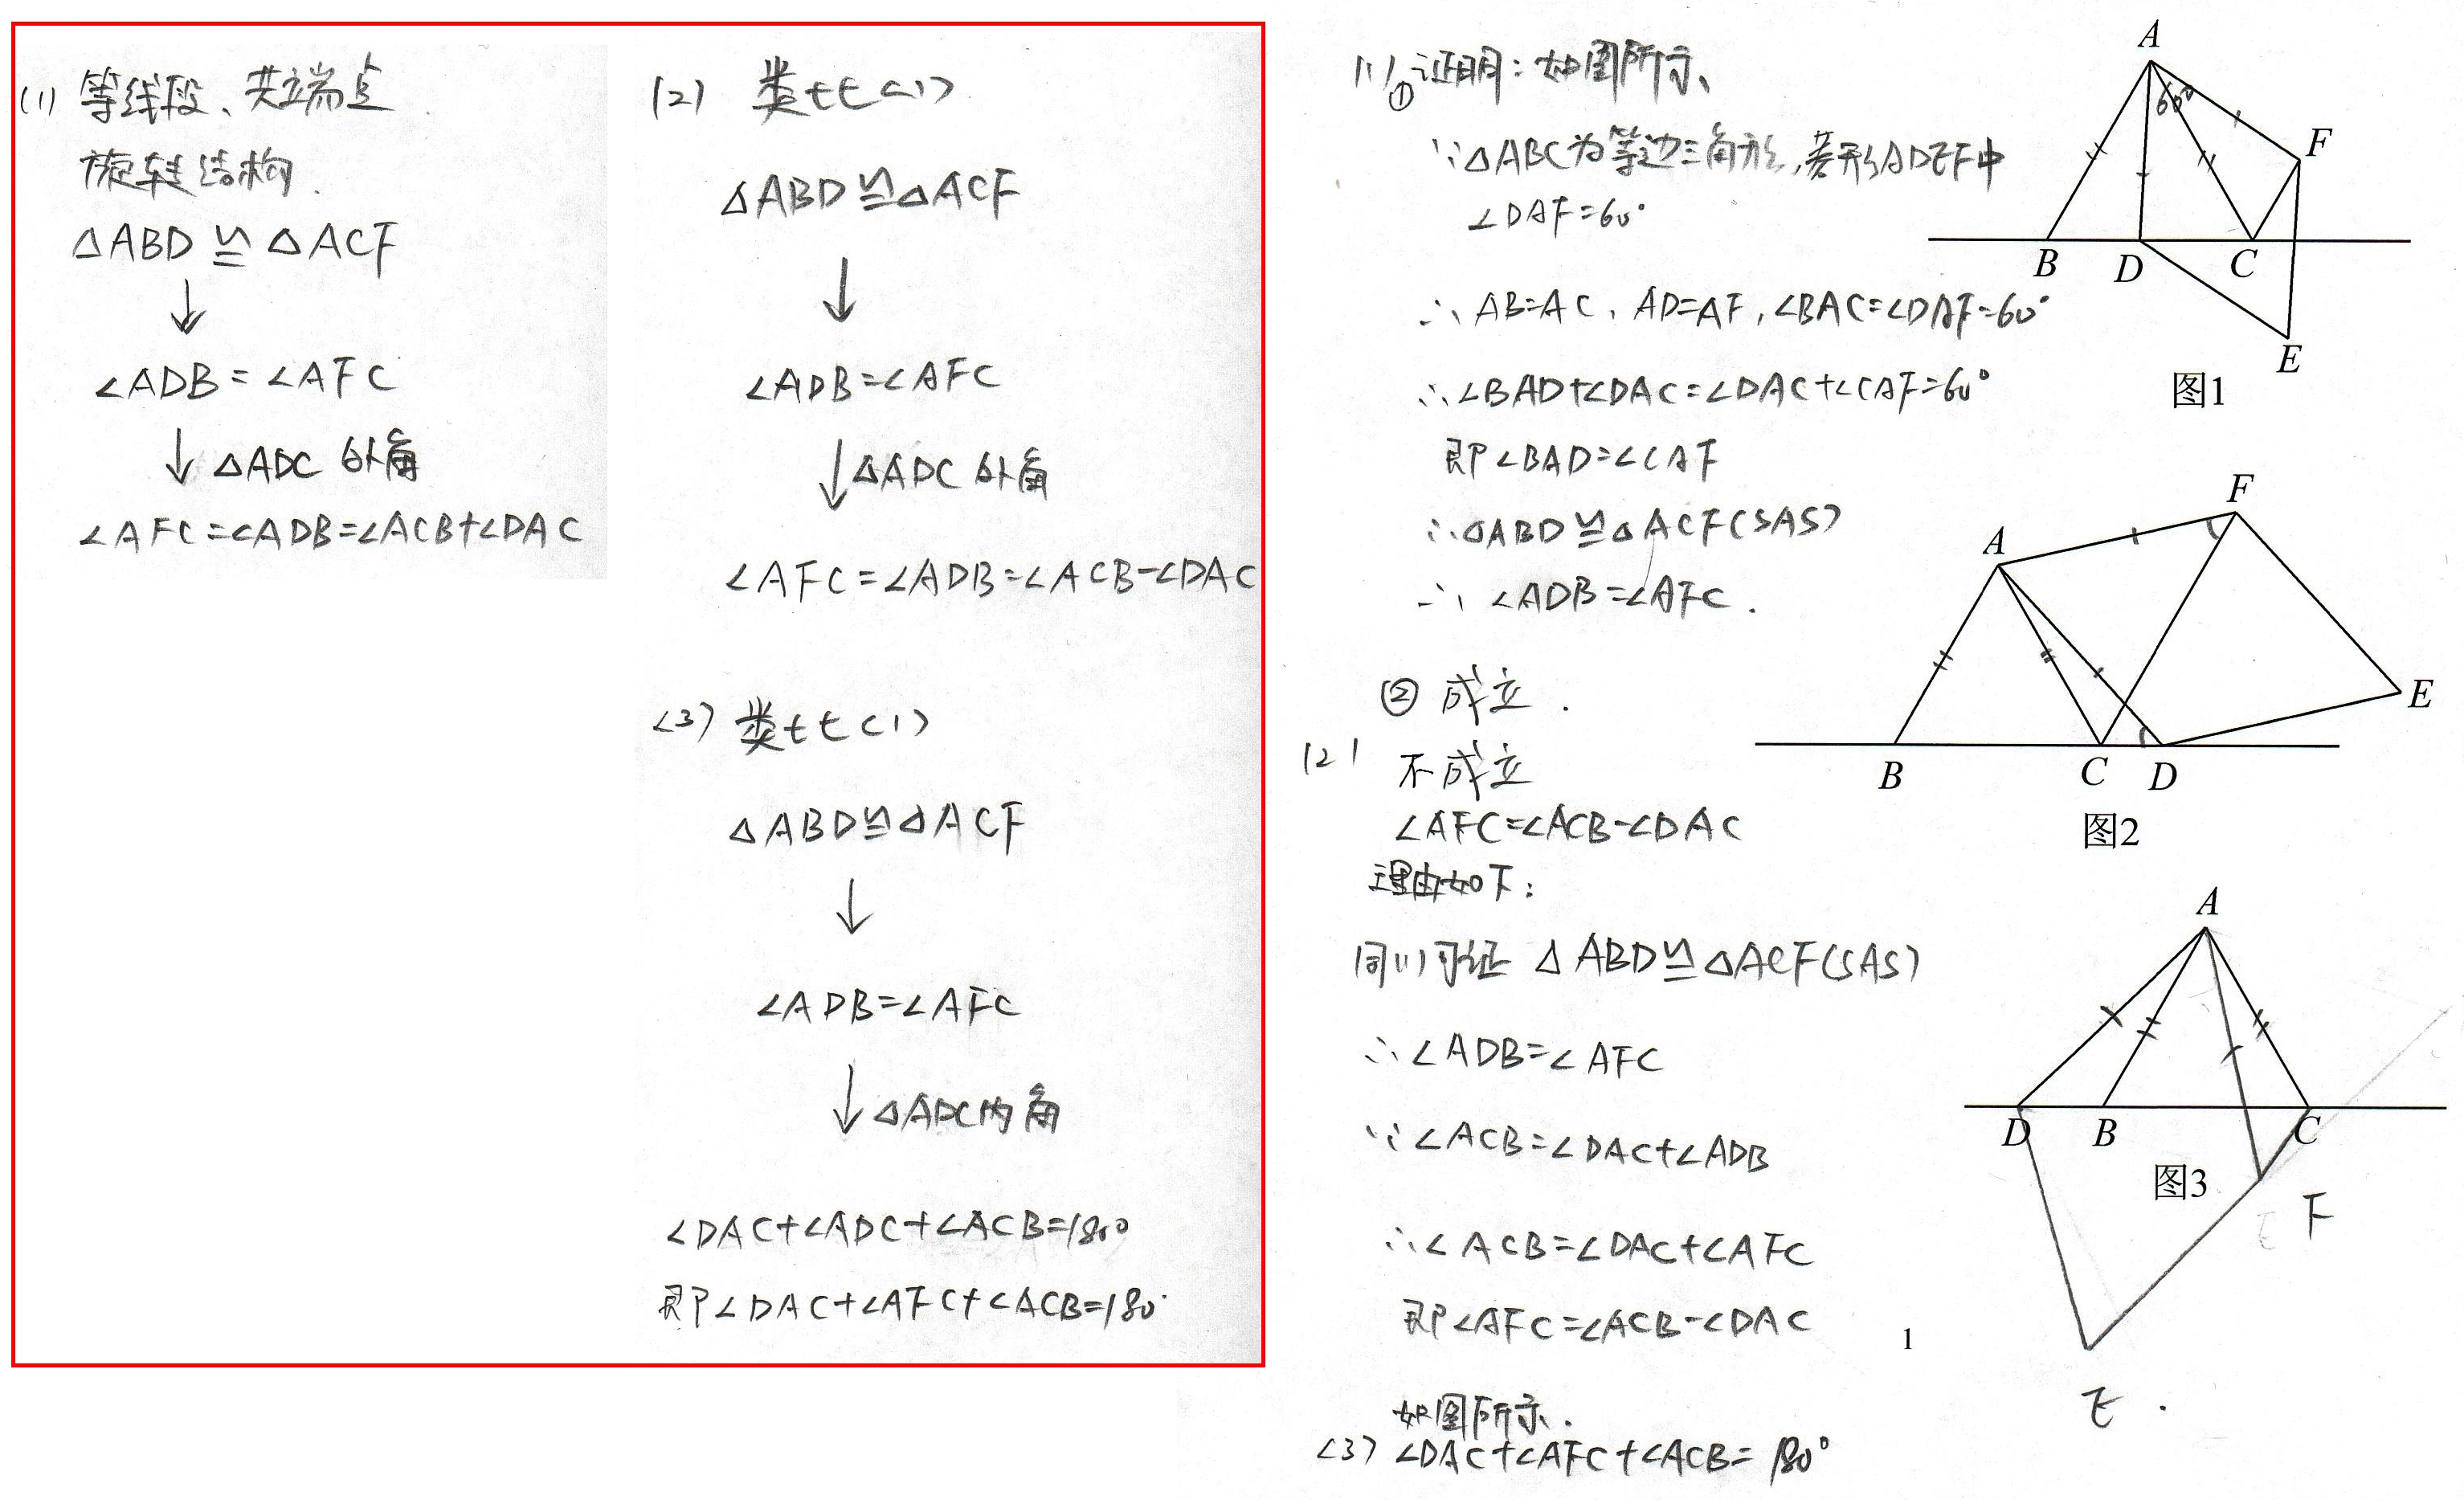
\includegraphics[width=.95\textwidth]{T22-A01-04-04-Ans.jpg}
\end{center}
\end{onlysolution}%
\end{defproblem}






\begin{defproblem}{T22-A01-05}%
\begin{onlyproblem}%
在$\triangle ABC$中,$\angle ACB$是锐角,点$D$在射线$BC$上运动,连接$AD$,将线段$AD$绕点$A$逆时针旋转90$^{\circ }$,得到$AE$,连接$EC$.

(1)操作发现:若$AB=AC$,$\angle BAC =90^{\circ }$,当$D$在线段$BC$上时(不与点$B$重合),如图1所示,请你直接写出线段$CE$和$BD$的位置关系是{\_}{\_}{\_}{\_}{\_}{\_}{\_}{\_},数量关系是{\_}{\_}{\_}{\_}{\_}{\_}{\_}{\_}{\_}{\_};

(2)猜想论证:在(1)的条件下,当$D$在线段$BC$的延长线上时,如图2所示,请你判断(1)中结论是否成立,并证明你的判断;

(3)拓展延伸:如图3,若$AB \ne  AC$,$\angle  BAC \ne 90^{\circ }$,点$D$在线段$BC$上运动,试探究:当锐角$\angle  ACB$等于{\_}{\_}{\_}{\_}{\_}度时,线段$CE$和$BD$之间的位置关系仍成立(点$C$,$E$重合除外)?此时若作$DF \bot  AD$交线段$CE$于点$F$,且当$AC=3\sqrt 2 $时,请直接写出线段$CF$的长的最大值是{\_}{\_}{\_}{\_}{\_}{\_}.

\begin{center}
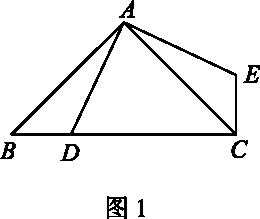
\includegraphics[scale=0.8]{T22-A01-05-01.pdf}\qquad
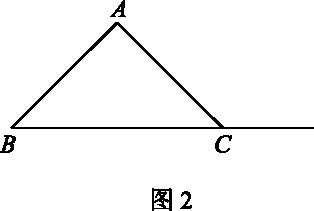
\includegraphics[scale=0.8]{T22-A01-05-02.pdf}\qquad
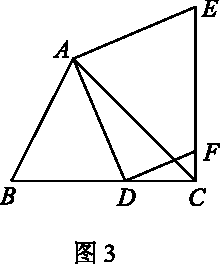
\includegraphics[scale=0.8]{T22-A01-05-03.pdf}
\end{center}
% \begin{flushright}
% 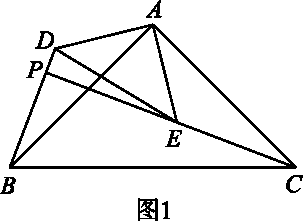
\includegraphics[scale=0.8]{T22-A01-02-01.pdf}\\
% 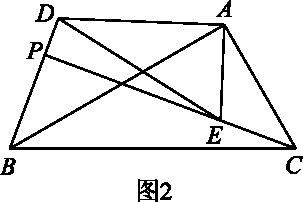
\includegraphics[scale=0.8]{T22-A01-02-02.pdf}\\
% 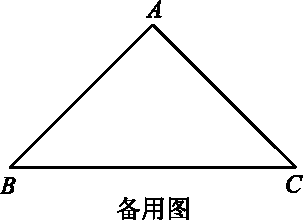
\includegraphics[scale=0.8]{T22-A01-02-03.pdf}
% \end{flushright}

\end{onlyproblem}%
\begin{onlysolution}%
\begin{center}
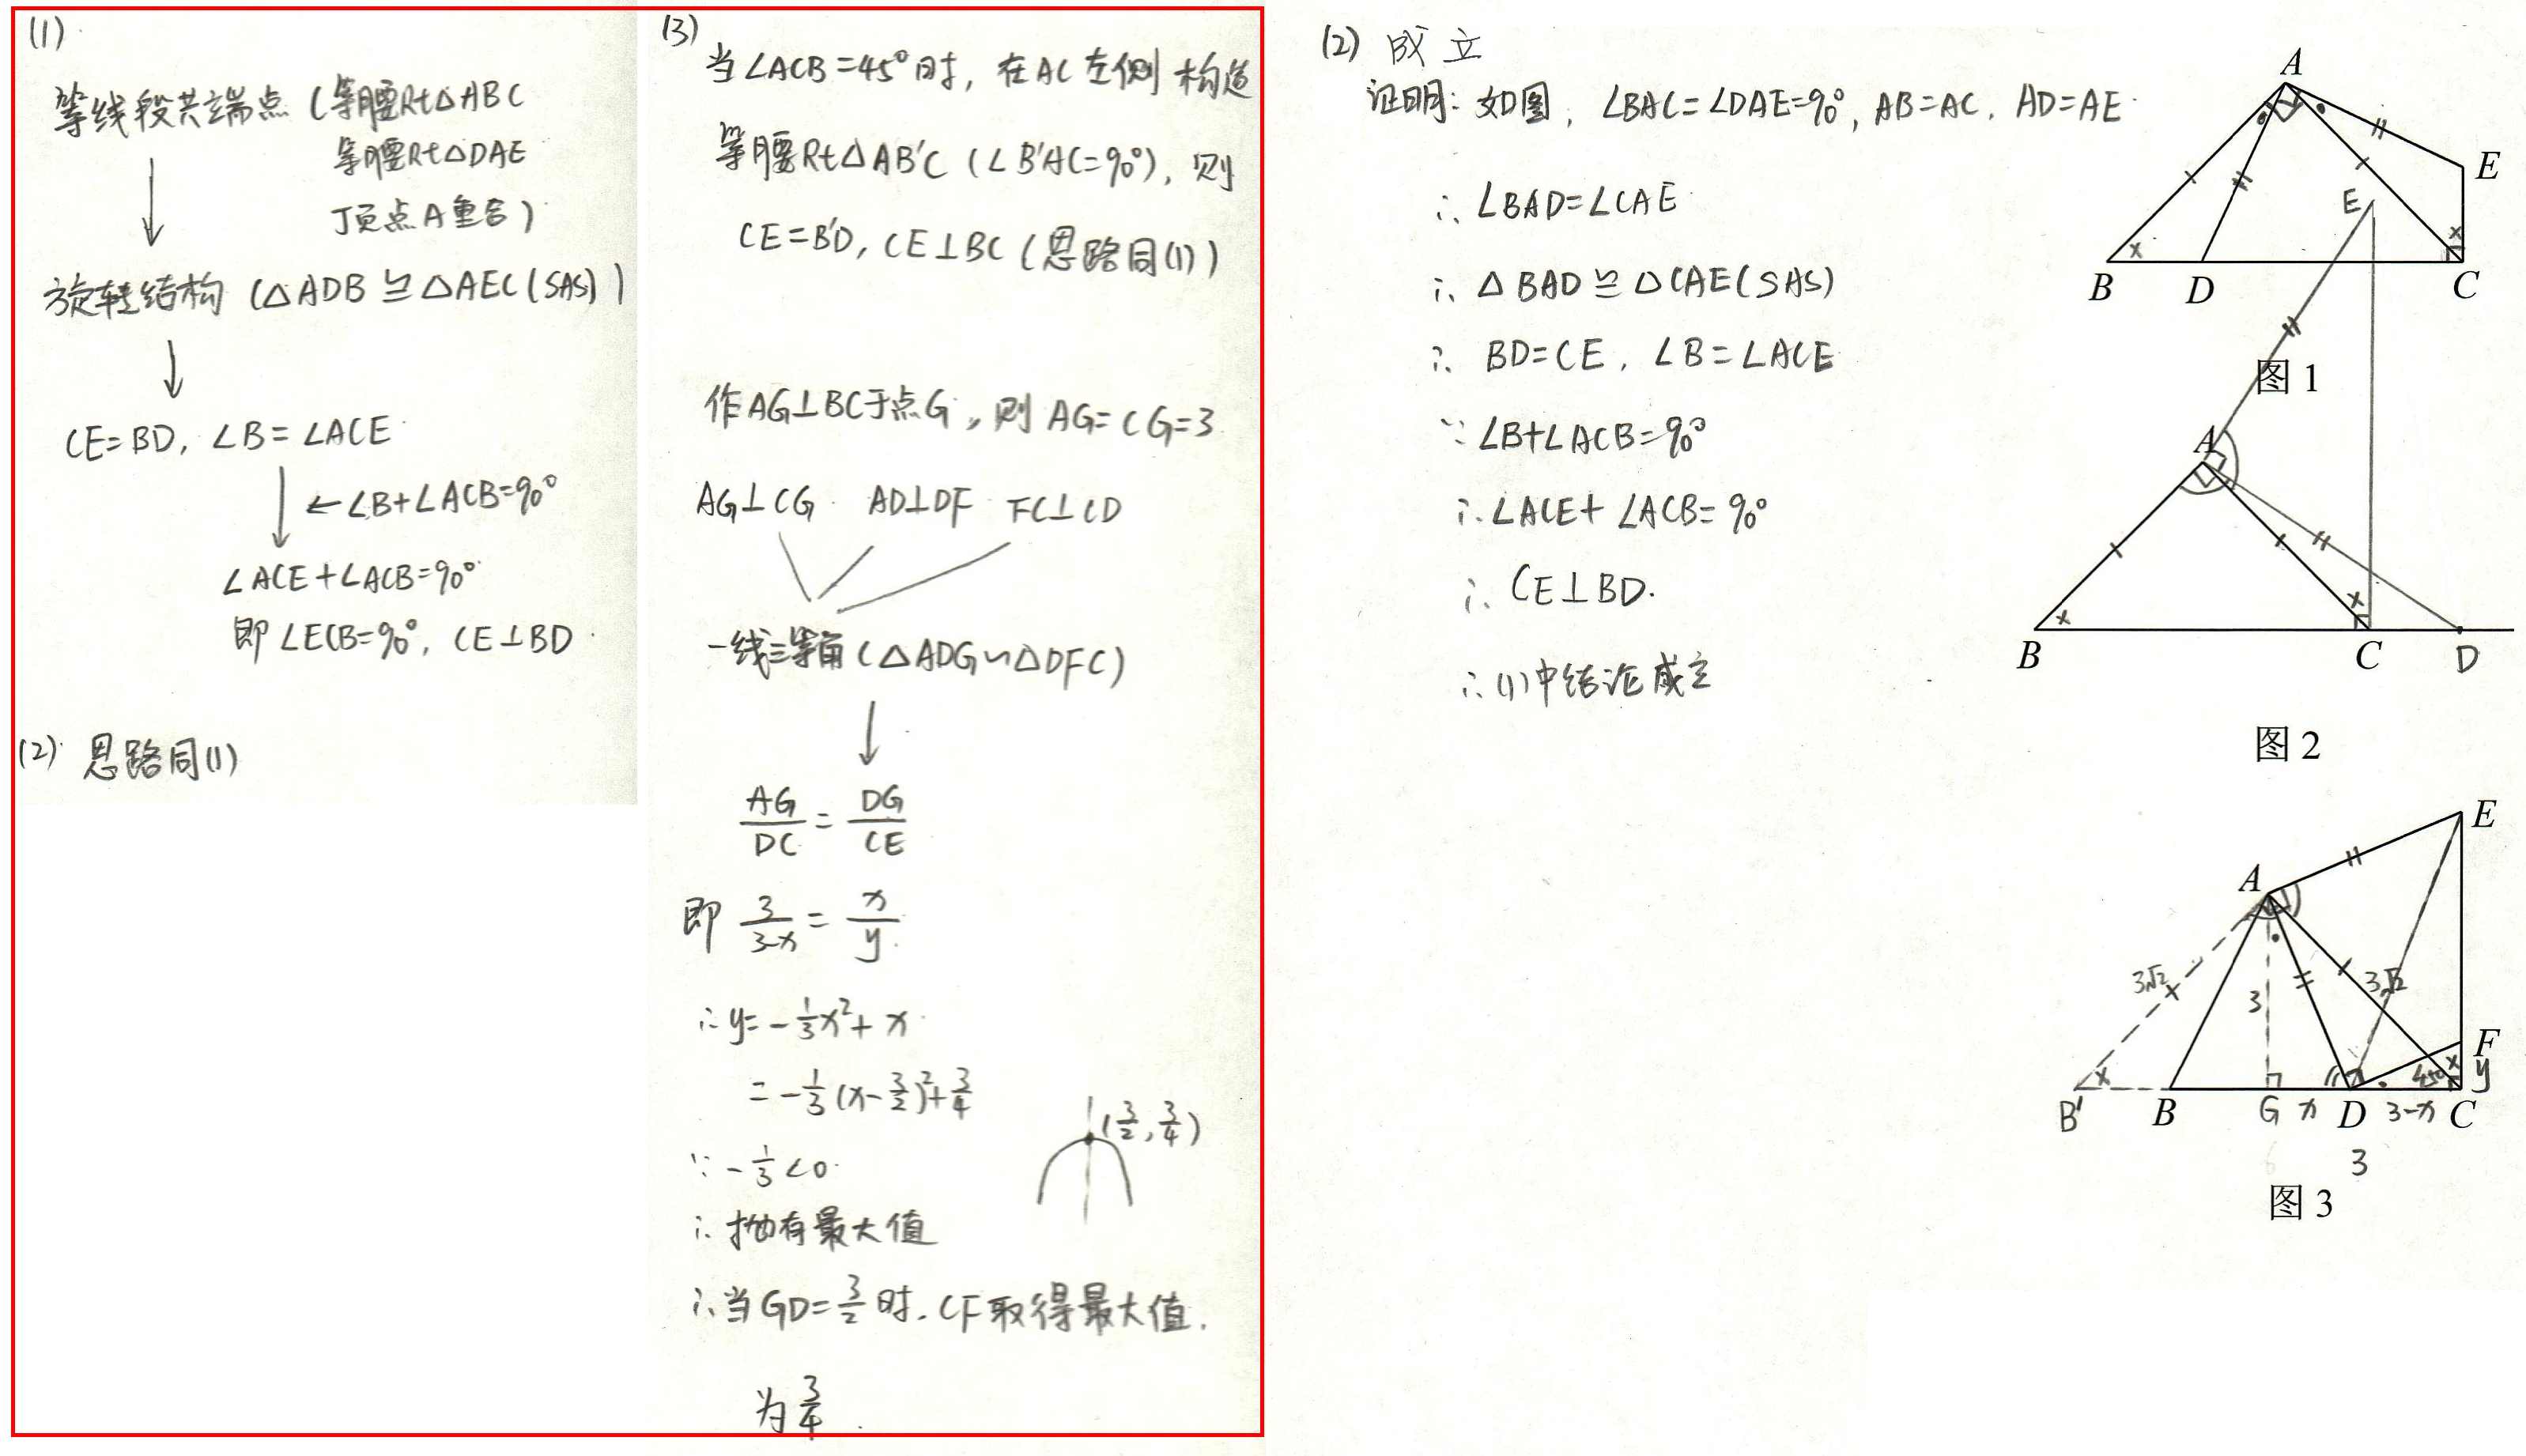
\includegraphics[width=.95\textwidth]{T22-A01-05-04-Ans.jpg}
\end{center}
\end{onlysolution}%
\end{defproblem}






\begin{defproblem}{T22-A01-06}%
\begin{onlyproblem}%
\href{run:./ItemBankFigures/T22-A01-06.ggb}{(查看动态演示)}
如图1,四边形$ABCD$是正方形,点$E$是$AB$边的中点,以$AE$为边作正方形$AEFG$,连接$DE$,$BG$.

(1)发现

①线段$DE$,$BG$之间的数量关系是{\_}{\_}{\_}{\_}{\_}{\_}{\_}{\_}{\_}{\_}{\_}{\_}{\_}{\_};

②直线$DE$,$BG$之间的位置关系是{\_}{\_}{\_}{\_}{\_}{\_}{\_}{\_}{\_}{\_}{\_}{\_}{\_}{\_}.

(2)探究

如图2,将正方形$AEFG$绕点$A$逆时针旋转,(1)中的结论是否仍然成立?若成立,请给出证明;若不成立,请说明理由.

(3)应用

如图3,将正方形$AEFG$绕点$A$逆时针旋转一周,记直线$DE$与$BG$的交点为$P$,若$AB=4$,请直接写出点$P$到$CD$所在直线距离的最大值和最小值.

\begin{center}
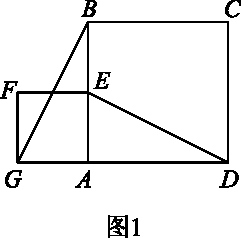
\includegraphics[scale=0.8]{T22-A01-06-01.pdf}\qquad
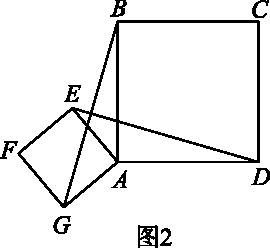
\includegraphics[scale=0.8]{T22-A01-06-02.pdf}\qquad
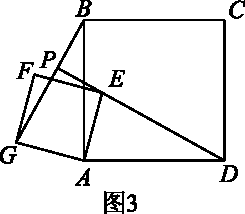
\includegraphics[scale=0.8]{T22-A01-06-03.pdf}
\end{center}


% \begin{flushright}
% 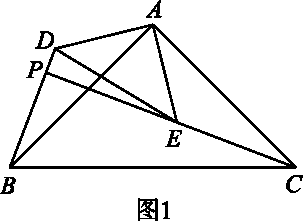
\includegraphics[scale=0.8]{T22-A01-02-01.pdf}\\
% 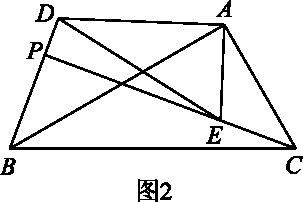
\includegraphics[scale=0.8]{T22-A01-02-02.pdf}\\
% 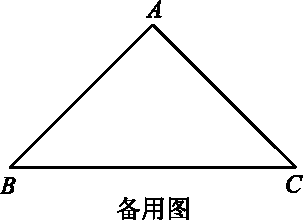
\includegraphics[scale=0.8]{T22-A01-02-03.pdf}
% \end{flushright}

\end{onlyproblem}%
\begin{onlysolution}%
\begin{center}
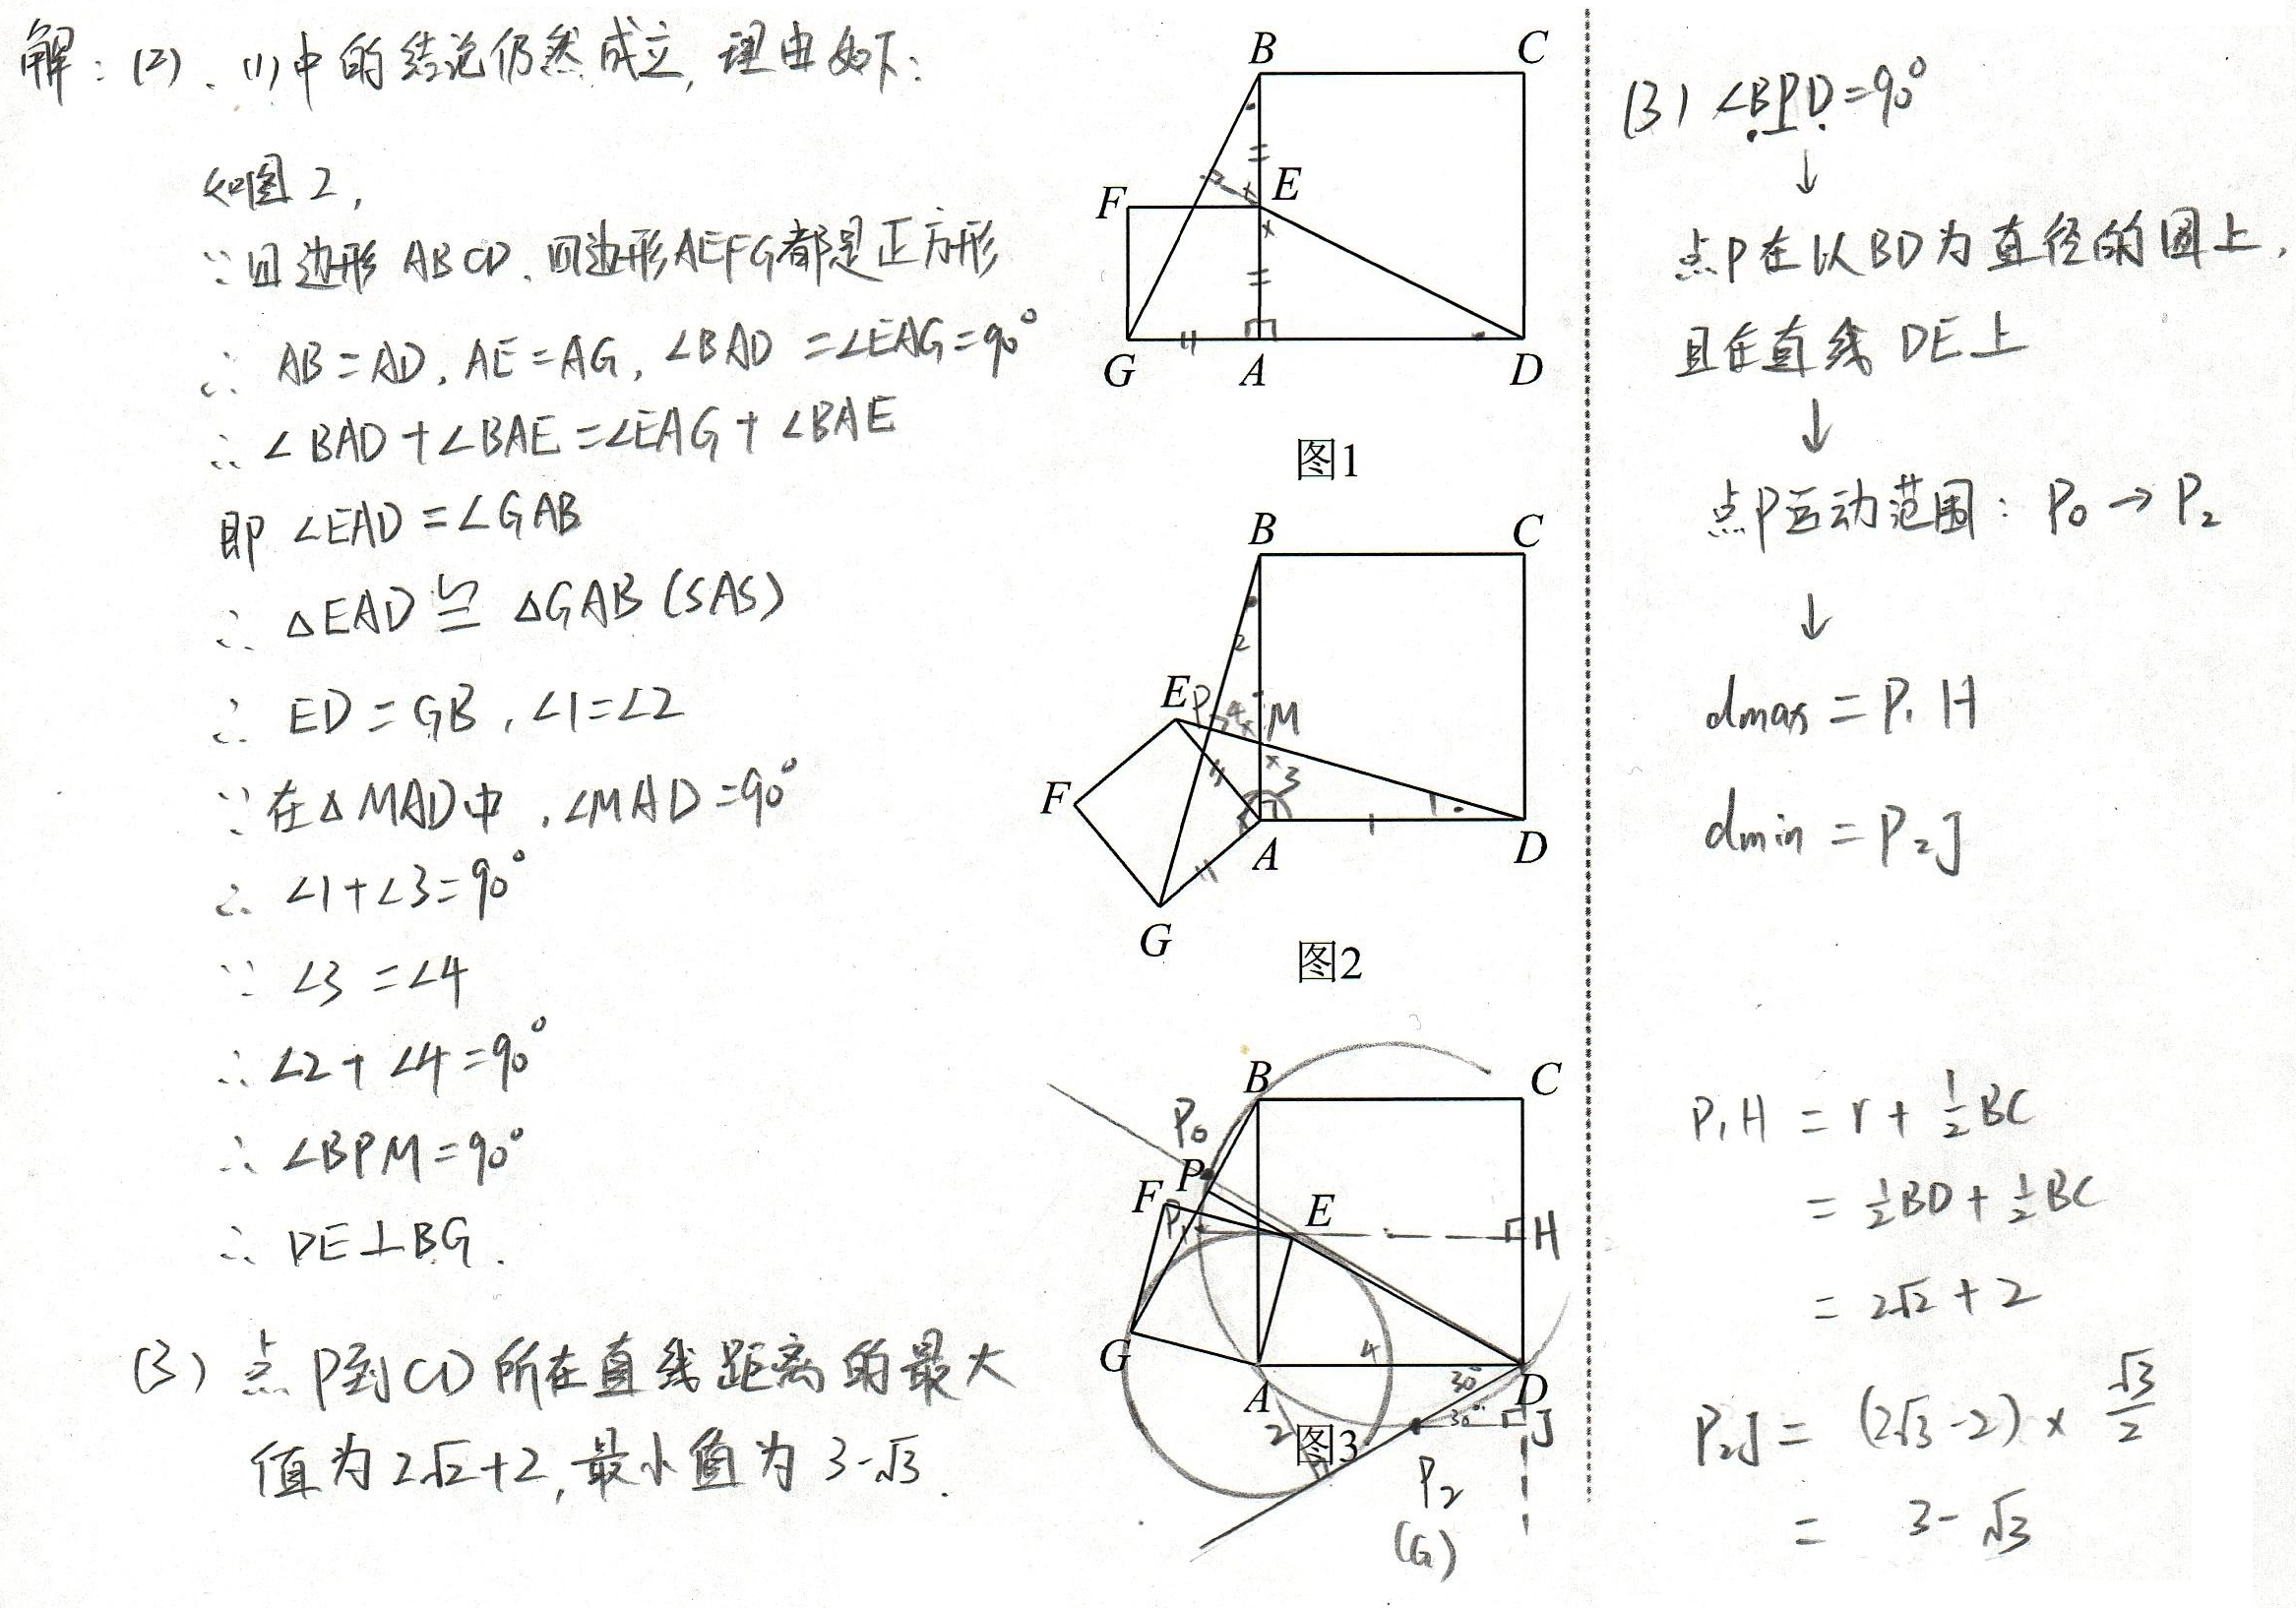
\includegraphics[width=.95\textwidth]{T22-A01-06-04-Ans.jpg}
\end{center}
\end{onlysolution}%
\end{defproblem}






\begin{defproblem}{T22-A01-07}%
\begin{onlyproblem}%
% \href{run:./ItemBankFigures/T22-A01-06.ggb}{(查看动态演示)}
如图1,点$E$为正方形$ABCD$边$ CB$延长线上一点,在$\triangle BEF$中,$\angle BEF=90^{\circ }$,$EF=BE$,连接$DF$.取$DF$的中点$G$,连接$CG$,$EG$,易证$CG=EG$且$CG\bot EG$.

(1)如图2,将$\triangle BEF$绕点$B$顺时针旋转,使$BE$落在$AB$边上,此时点$F$恰好落在$BD$上,其他条件不变,则线段$CG$,$EG$有怎样的数量关系和位置关系?请写出你的猜想,并加以证明.

(2)如图3,将$\triangle BEF$绕点$B$逆时针旋转90$^{\circ }$,其他条件不变.若$AB=3$,$BE=1$,请直接写出$CG$的长.

\begin{center}
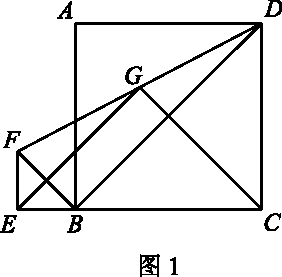
\includegraphics[scale=0.8]{T22-A01-07-01.pdf}\qquad
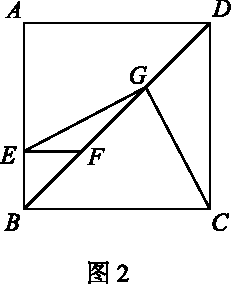
\includegraphics[scale=0.8]{T22-A01-07-02.pdf}\qquad
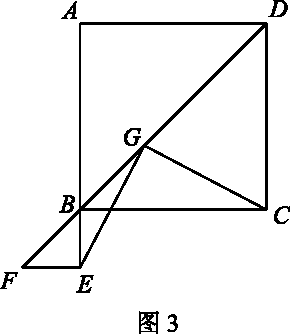
\includegraphics[scale=0.8]{T22-A01-07-03.pdf}
\end{center}


% \begin{flushright}
% 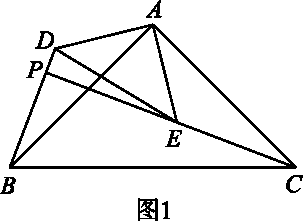
\includegraphics[scale=0.8]{T22-A01-02-01.pdf}\\
% 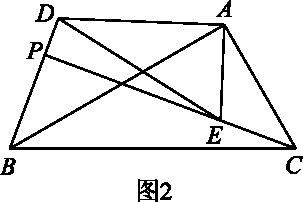
\includegraphics[scale=0.8]{T22-A01-02-02.pdf}\\
% 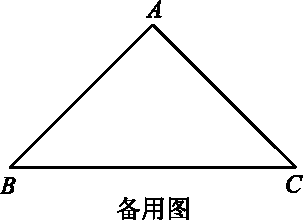
\includegraphics[scale=0.8]{T22-A01-02-03.pdf}
% \end{flushright}

\end{onlyproblem}%
\begin{onlysolution}%
(1)$CG=EG$且$CG \bot  EG$,证明略.

(2)$\sqrt 5 $.

做题要求:

1.读题标注,保留做题痕迹;

2.对比分析,写出不变结构;

3.梳理路线图,并类比解决问题.

分析不变特征:
①对比图1,图2中的条件,
发现\underline{\hspace*{2cm}}是不变特征;

②考虑\underline{\hspace*{2cm}}与\underline{\hspace*{2cm}}组合,形成不变结构;

③类比此结构解决问题.

路线图(示例):

\underline{\hspace*{2cm}}是中点,且\underline{\hspace*{1cm}}//\underline{\hspace*{1cm}},考虑\underline{\hspace*{2cm}}。

辅助线:


\begin{center}
% 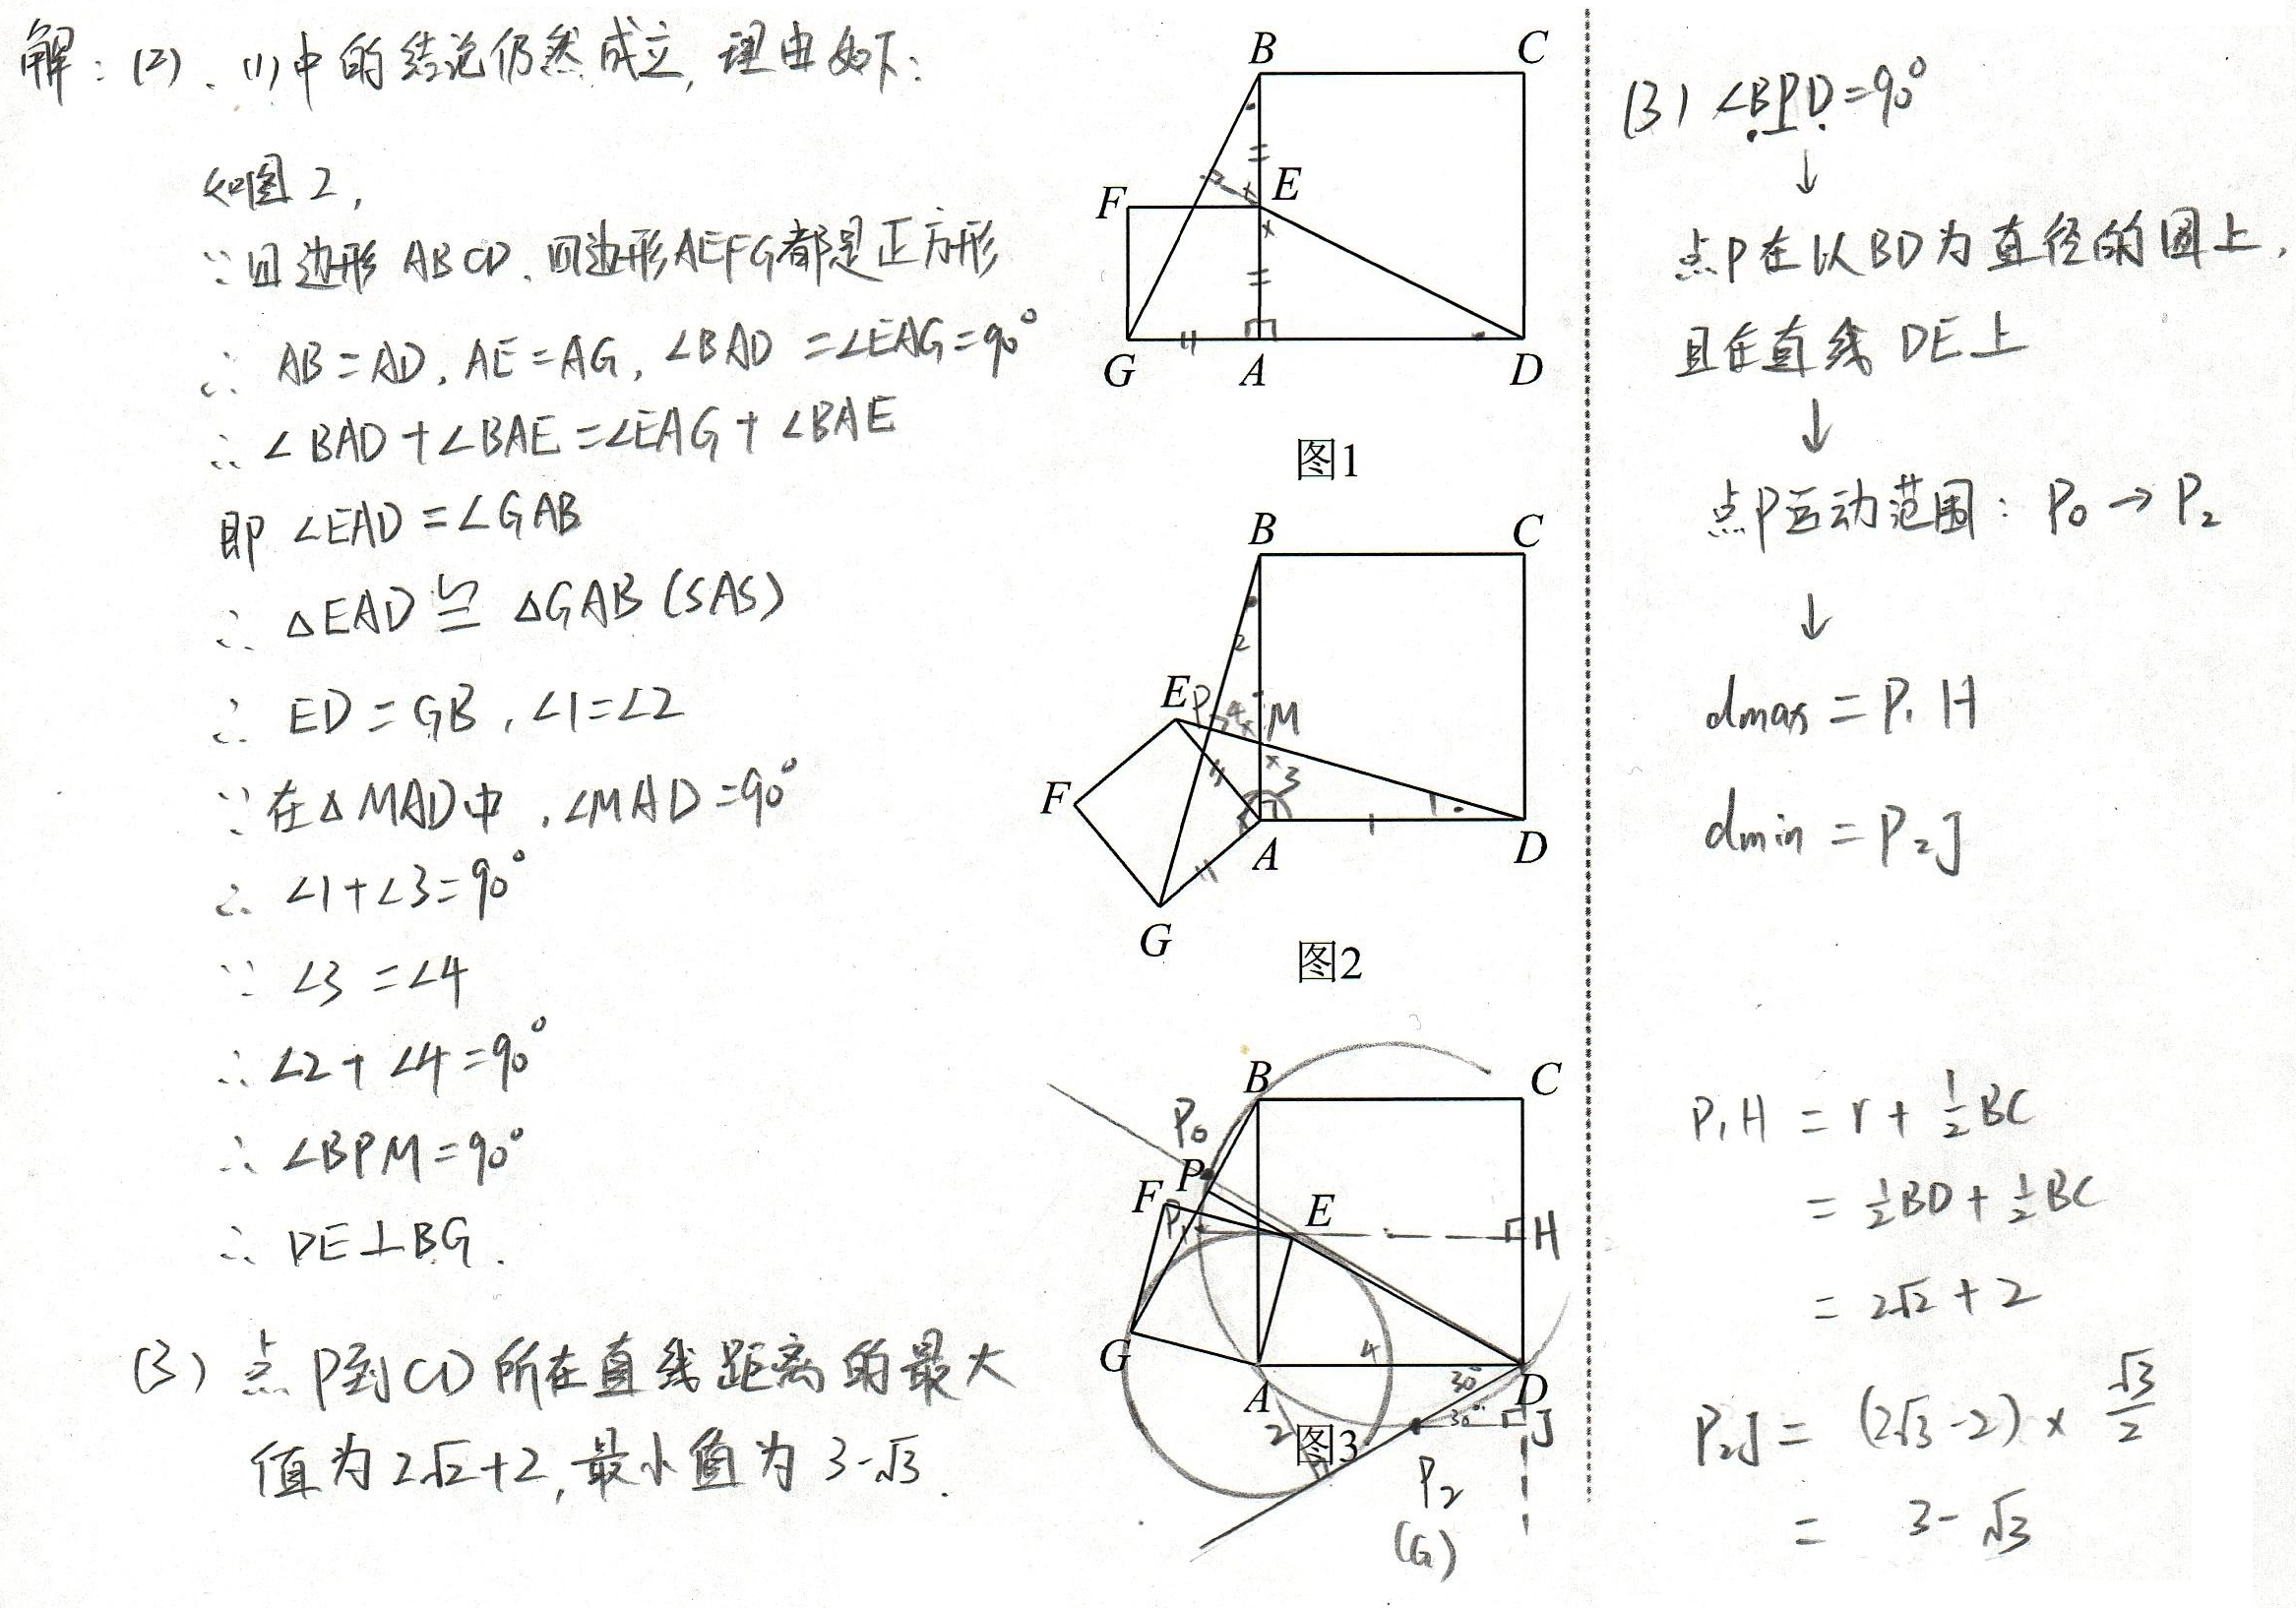
\includegraphics[width=.95\textwidth]{T22-A01-06-04-Ans.jpg}
\end{center}
\end{onlysolution}%
\end{defproblem}






\begin{defproblem}{T22-A01-08}%
\begin{onlyproblem}%
% \href{run:./ItemBankFigures/T22-A01-06.ggb}{(查看动态演示)}
已知,在$\triangle ABC$中,$\angle BAC=90^{\circ }$,$\angle ABC=45^{\circ }$,$D$为直线$BC$上一动点(不与点$B$,$C$重合),以$AD$为边作正方形$ADEF$,连接$CF$.

(1)如图1,当点$D$在线段$BC$上时,求证:$BC=CF+CD$.

(2)如图2,当点$D$在线段$BC$的延长线上时,其他条件不变,请直接写出$BC$,$CD$,$CF$三条线段之间的数量关系.

(3)如图3,当点$D$在线段$BC$的反向延长线上时,点$A$,$F$分别在直线$BC$的两侧,其他条件不变.

①请直接写出$BC$,$CD$,$CF$三条线段之间的数量关系;

②若正方形$ADEF$的边长为$2\sqrt 2$,对角线$AE$,$DF$相交于点$O$,求$OC$的长.


\begin{center}
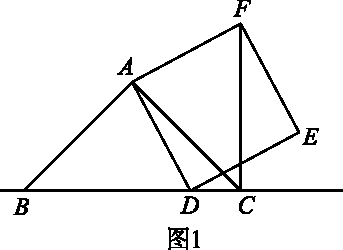
\includegraphics[scale=0.8]{T22-A01-08-01.pdf}\qquad
\includegraphics[scale=0.8]{T22-A01-08-02.pdf}\qquad
\includegraphics[scale=0.8]{T22-A01-08-03.pdf}
\end{center}


% \begin{flushright}
% \includegraphics[scale=0.8]{T22-A01-02-01.pdf}\\
% \includegraphics[scale=0.8]{T22-A01-02-02.pdf}\\
% \includegraphics[scale=0.8]{T22-A01-02-03.pdf}
% \end{flushright}

\end{onlyproblem}%
\begin{onlysolution}%
(1)证明略.
提示:题目中有旋转结构,证明$\triangle ABD\cong \triangle ACF$(SAS),
得到$BD=CF$,进而得证.

(2)$BC=CF-CD$.

(3)① $BC=CD-CF$;② $OC=2$.
	

\begin{center}
% \includegraphics[width=.95\textwidth]{T22-A01-06-04-Ans.jpg}
\end{center}
\end{onlysolution}%
\end{defproblem}






\begin{defproblem}{T22-A01-09}%
\begin{onlyproblem}%
% \href{run:./ItemBankFigures/T22-A01-06.ggb}{(查看动态演示)}
(2018年河南中考)

(1)问题发现

如图1,在$\triangle OAB$和$\triangle OCD$中,$OA=OB$,$OC=OD$,$\angle AOB=\angle COD=40^{\circ }$,连接$AC$,$BD$交于点$M$.填空:

①$\dfrac{AC}{BD}$的值为{\_}{\_}{\_}{\_}{\_}{\_}{\_}{\_}{\_}{\_}{\_}{\_}{\_};
②$\angle AMB$的度数为{\_}{\_}{\_}{\_}{\_}{\_}{\_}{\_}{\_}{\_}{\_}{\_}{\_}.

(2)类比探究

如图2,在$\triangle OAB$和$\triangle OCD$中,$\angle AOB=\angle COD=90^{\circ }$,$\angle OAB=\angle OCD=30^{\circ }$,连接$AC$交$BD$的延长线于点$M$.请判断$\dfrac{AC}{BD}$的值及$\angle AMB$的度数,并说明理由.

(3)拓展延伸

在(2)的条件下,将$\triangle OCD$绕点$O$在平面内旋转,$AC$,$BD$所在直线交于点$M$.若$OD=1$,$OB=\sqrt 7 $,请直接写出当点$C$与点$M$重合时$AC$的长.


\begin{center}
\includegraphics[scale=0.8]{T22-A01-09-01.pdf}\qquad
\includegraphics[scale=0.8]{T22-A01-09-02.pdf}\qquad
\includegraphics[scale=0.8]{T22-A01-09-03.pdf}
\end{center}


% \begin{flushright}
% \includegraphics[scale=0.8]{T22-A01-02-01.pdf}\\
% \includegraphics[scale=0.8]{T22-A01-02-02.pdf}\\
% \includegraphics[scale=0.8]{T22-A01-02-03.pdf}
% \end{flushright}

\end{onlyproblem}%
\begin{onlysolution}%
(1)①1;②40$^{\circ }$;

(2)$\dfrac{AC}{BD}=\sqrt 3 $,$\angle AMB=90^{\circ }$,理由略;
\begin{center}
% \includegraphics[width=.95\textwidth]{T22-A01-06-04-Ans.jpg}
\end{center}
\end{onlysolution}%
\end{defproblem}


\begin{defproblem}{T22-A01-10}%
\begin{onlyproblem}%
% \href{run:./ItemBankFigures/T22-A01-06.ggb}{(查看动态演示)}
(2017年河南中考)
如图1,在Rt$\triangle ABC$中,$\angle  A =90 ^{\circ }$,$AB=AC$,点$D$,$E$分别在边$AB$,$AC$上,$AD=AE$,连接$DC$,点$M$,$P$,$N$分别为$DE$,$DC$,$BC$的中点.

(1)观察猜想

图1中,线段$PM$与$PN$的数量关系是{\_}{\_}{\_}{\_}{\_}{\_}{\_}{\_}{\_}{\_}{\_},位置关系是{\_}{\_}{\_}{\_}{\_}{\_}{\_}{\_}{\_};

(2)探究证明

把$\triangle ADE$绕点$A$逆时针方向旋转到图2的位置,连接$MN$,$BD$,$CE$,判断$\triangle PMN$的形状,并说明理由;

(3)拓展延伸

把$\triangle ADE$绕点$A$在平面内自由旋转,若$AD=4$,$AB=10$,请直接写出$\triangle PMN$面积的最大值.


\begin{center}
\includegraphics[scale=0.8]{T22-A01-10-01.pdf}\qquad
\includegraphics[scale=0.8]{T22-A01-10-02.pdf}
\end{center}


% \begin{flushright}
% \includegraphics[scale=0.8]{T22-A01-02-01.pdf}\\
% \includegraphics[scale=0.8]{T22-A01-02-02.pdf}\\
% \includegraphics[scale=0.8]{T22-A01-02-03.pdf}
% \end{flushright}

\end{onlyproblem}%
\begin{onlysolution}%
(1)$PM=PN$;$PM \bot  PN$;

(2)$\triangle PMN$为等腰直角三角形,理由略;

(3)$\triangle PMN$面积的最大值为$\dfrac{49}{2}$.
\begin{center}
% \includegraphics[width=.95\textwidth]{T22-A01-06-04-Ans.jpg}
\end{center}
\end{onlysolution}%
\end{defproblem}







\begin{defproblem}{T22-A01-11}%
\begin{onlyproblem}%
% \href{run:./ItemBankFigures/T22-A01-06.ggb}{(查看动态演示)}
(2018--2019学年下学期九年级二模)
现有正方形$ABCD$和一个以$O$为直角顶点的三角板,移动三角板,使三角板的两直角边所在直线分别与直线$BC$,$CD$交于点$M$,$N$.

如图1,若点$O$与点$A$重合,容易得到线段$OM$与$ON$的关系.

(1)观察猜想:如图2,若点$O$在正方形的中心(即两条对角线的交点),$OM$与$ON$的数量关系是{\_}{\_}{\_}{\_}{\_}{\_}{\_}{\_}{\_}{\_}{\_};

(2)探究证明:如图3,若点$O$在正方形的内部(含边界),且$OM=ON$,请判断三角板移动过程中所有满足条件的点$O$可组成什么图形,并说明理由;

(3)拓展延伸:若点$O$在正方形的外部,且$OM=ON$,请你在图4中画出满足条件的一种情况,并就``三角板在各种情况下(含外部)移动,所有满足条件的点$O$所组成的图形'',写出正确的结论.(不必说明理由)



\begin{center}
\includegraphics[scale=0.8]{T22-A01-11-01.pdf}\qquad
\includegraphics[scale=0.8]{T22-A01-11-02.pdf}\qquad
\includegraphics[scale=0.8]{T22-A01-11-03.pdf}\qquad
\includegraphics[scale=0.8]{T22-A01-11-04.pdf}
\end{center}


% \begin{flushright}
% \includegraphics[scale=0.8]{T22-A01-02-01.pdf}\\
% \includegraphics[scale=0.8]{T22-A01-02-02.pdf}\\
% \includegraphics[scale=0.8]{T22-A01-02-03.pdf}
% \end{flushright}

\end{onlyproblem}%
\begin{onlysolution}%
\begin{center}
\includegraphics[width=.95\textwidth]{T22-A01-11-05-Ans.jpg}
\end{center}
\end{onlysolution}%
\end{defproblem}





\begin{defproblem}{T22-A01-12}%
\begin{onlyproblem}%
% \href{run:./ItemBankFigures/T22-A01-06.ggb}{(查看动态演示)}
(2017--2018学年下学期九年级二模)
\textbf{问题发现}:如图1,在$\triangle ABC$中,$\angle  C =90 ^{\circ }$,分别以$AC$,$BC$为边向外侧作正方形$ACDE$和正方形$BCFG$.

(1)$\triangle ABC$和$\triangle DCF$面积的关系是{\_}{\_}{\_}{\_}{\_}{\_}{\_}{\_}{\_}{\_}{\_}{\_}{\_}{\_};(请在横线上填写``相等''或``不相等'')

(2)\textbf{拓展探究}:若$\angle  C \ne 90^{\circ }$,(1)中的结论还成立吗?若成立,请结合图2给出证明;若不成立,请说明理由;

(3)\textbf{解决问题}:如图3,在四边形$ABCD$中,$AC \bot BD$,且$AC$与$BD$的和为10,分别以四边形$ABCD$的四条边为边向外侧作正方形$ABFE$、正方形$BCHG$、正方形$CDJI$,正方形$DALK$,运用(2)的结论,图中阴影部分的面积和是否有最大值?如果有,请求出最大值,如果没有,请说明理由.


\begin{center}
\includegraphics[scale=0.8]{T22-A01-12-01.pdf}\qquad
\includegraphics[scale=0.8]{T22-A01-12-02.pdf}\qquad
\includegraphics[scale=0.8]{T22-A01-12-03.pdf}
\end{center}


% \begin{flushright}
% \includegraphics[scale=0.8]{T22-A01-02-01.pdf}\\
% \includegraphics[scale=0.8]{T22-A01-02-02.pdf}\\
% \includegraphics[scale=0.8]{T22-A01-02-03.pdf}
% \end{flushright}

\end{onlyproblem}%
\begin{onlysolution}%
\begin{center}
% \includegraphics[width=.95\textwidth]{T22-A01-12-05-Ans.jpg}
\end{center}
\end{onlysolution}%
\end{defproblem}



\begin{defproblem}{T22-A01-13}%
\begin{onlyproblem}%
% \href{run:./ItemBankFigures/T22-A01-06.ggb}{(查看动态演示)}
(2016年河南中考)
如图1,在Rt$ABC$中,$\angle  ACB =90 ^{\circ }$,$\angle  B =60 ^{\circ }$,$D$为$AB$的中点,$\angle  EDF =90 ^{\circ }$,$DE$交$AC$于点$G$,$DF$经过点$C$.

(1)求$\angle  ADE$的度数;

(2)如图2,将图1中的$\angle EDF$绕点$D$顺时针方向旋转角$\alpha (0^{\circ }<\alpha <60^{\circ })$,旋转过程中的任意两个位置分别记为$\angle E_{1}DF_{1}$,$\angle E_{2}DF_{2}$,$DE_{1}$交直线$AC$于点$P$,$DF_{1}$交直线$BC$于点$Q$,$DE_{2}$交直线$AC$于点$M$,$DF_{2}$交直线$BC$于点$N$,求$\dfrac{PM}{QN}$的值;

(3)若图1中的$\angle B=\beta (60^{\circ }<\beta <90^{\circ })$,(2)中的其余条件不变,请直接写出$\dfrac{PM}{QN}$的值(用含$\beta$的式子表示).

\begin{center}
\includegraphics[scale=0.8]{T22-A01-13-01.pdf}\qquad
\includegraphics[scale=0.8]{T22-A01-13-02.pdf}
\end{center}


% \begin{flushright}
% \includegraphics[scale=0.8]{T22-A01-02-01.pdf}\\
% \includegraphics[scale=0.8]{T22-A01-02-02.pdf}\\
% \includegraphics[scale=0.8]{T22-A01-02-03.pdf}
% \end{flushright}

\end{onlyproblem}%
\begin{onlysolution}%
\begin{center}
% \includegraphics[width=.95\textwidth]{T22-A01-12-05-Ans.jpg}
\end{center}
\end{onlysolution}%
\end{defproblem}






\begin{defproblem}{T22-A01-14}%
\begin{onlyproblem}%
(1)问题发现 如图1,在Rt$\triangle ABC$中,$\angle ACB=90^{\circ}$,$\angle A=30^{\circ}$,点$D$,$E$分别在边$AB$,$AC$上,$DE\bot AB$,连接$BE$,点$F$为$BE$的中点.

填空:①$DF$与$CF$的数量关系是{\_}{\_}{\_}{\_}{\_}{\_}{\_}{\_};②$\angle DFC=${\_}{\_}{\_}{\_}{\_}{\_}{\_}{\_}{\_}{\_}{\_}{\_}.

(2)类比探究 把Rt$\triangle ADE$绕点$A$旋转到图2的位置,请判断$DF$与$CF$的数量关系及$\angle DFC$的度数,并说明理由.

(3)拓展延伸 把Rt$\triangle ADE$绕点$A$在平面内自由旋转,若$BC=2$,$AE=\sqrt 3 $,请直接写出$DF$长度的最大值.

\vspace*{5\baselineskip}
\tabto{0.06\columnwidth}
\includegraphics[scale=.8]{\Newcurrentlabel.pdf}
\end{onlyproblem}%
\begin{onlysolution}%

\end{onlysolution}%
\end{defproblem}





\begin{defproblem}{T22-A01-15}%
\begin{onlyproblem}%
(2019)(10分)在$\triangle ABC$中,$CA=CB$,$\angle ACB=\alpha $.点$P$是平面内不与点$A$,$C$重合的任意一点.连接$AP$,将线段$AP$绕点$P$逆时针旋转$\alpha $得到线段$DP$,连接$AD$,$BD$,$CP$.

(1)\textbf{观察猜想}

如图1,当$\alpha =60^{\circ}$时,$\dfrac{BD}{CP}$的值是{\_}{\_}{\_}{\_}{\_}{\_}{\_}{\_}{\_}{\_},直线$BD$与直线$CP$相交所成的较小角的度数是{\_}{\_}{\_}{\_}{\_}{\_}{\_}{\_}{\_}{\_}.

(2)\textbf{类比探究}

如图2,当$\alpha =90^{\circ}$时,请写出$\dfrac{BD}{CP}$的值及直线$BD$与直线$CP$相交所成的较小角的度数,并就图2的情形说明理由.

(3)\textbf{解决问题}

当$\alpha =90^{\circ}$时,若点$E$,$F$分别是$CA$,$CB$的中点,点$P$在直线$EF$上,请直接写出点$C$,$P$,$D$在同一直线上时$\dfrac{AD}{CP}$的值.


\begin{tikzpicture}[scale=.5,line cap=round,line join=round]
% \tkzInit[xmax=14,ymax=10]
% \tkzClip[space=1]
\tkzDefPoint(0,0){A}
\tkzDefPoint(6,0){B}
\tkzDefPointBy[rotation=center B angle -60](A)
\tkzGetPoint{C}
\tkzDefPointBy[homothety=center A ratio 0.6](B)
\tkzGetPoint{DD}
\tkzDefPointBy[rotation=center A angle -20](DD)
\tkzGetPoint{D}
\tkzDefPointBy[rotation=center A angle 60](D)
\tkzGetPoint{P}

\tkzDrawPolygon[line width=0.4pt](A,B,C)
\tkzDrawPolygon[line width=0.4pt](A,D,P)
\tkzDrawSegments[line width=0.4pt](C,P B,D)


% \tkzDrawPoints(A)
% \tkzDrawPoints(B)
% \tkzDrawPoints(C)
% \tkzDrawPoints(D)
% \tkzDrawPoints(P)



\tkzLabelPoint[below](A){$A$}
\tkzLabelPoint[below](B){$B$}
\tkzLabelPoint[above](C){$C$}
\tkzLabelPoint[below](D){$D$}
\tkzLabelPoint[right](P){$P$}
\end{tikzpicture}
\begin{tikzpicture}[scale=.5]
% \tkzInit[xmax=14,ymax=10]
% \tkzClip[space=1]
\tkzDefPoint(0,0){A}
\tkzDefPoint(6,0){B}

\tkzCalcLength[cm](A,B)
\tkzGetLength{rAB}
\pgfmathparse{\rAB / sqrt(2)}
\edef\tkz@rb{\pgfmathresult}%
\tkzInterCC[R](A,\tkz@rb cm)(B,\tkz@rb cm)
\tkzGetFirstPoint{C}

\tkzDefPointBy[homothety=center A ratio 0.4](B)
\tkzGetPoint{DD}
\tkzDefPointBy[rotation=center A angle 80](DD)
\tkzGetPoint{D}

\tkzCalcLength[cm](A,D)
\tkzGetLength{rAD}
\pgfmathparse{\rAD / sqrt(2)}
\edef\tkz@rb{\pgfmathresult}%
\tkzInterCC[R](A,\tkz@rb cm)(D,\tkz@rb cm)
\tkzGetFirstPoint{P}
% \tkzGetPoint{P}

\tkzDrawPolygon[line width=0.4pt,line cap=round,line join=round](A,B,C)
\tkzDrawPolygon[line width=0.4pt,line cap=round,line join=round](A,D,P)
\tkzDrawSegments[line width=0.4pt](C,P B,D)

% \tkzDrawPoints(A)
% \tkzDrawPoints(B)
% \tkzDrawPoints(C)
% \tkzDrawPoints(D)
% \tkzDrawPoints(M)
% \tkzDrawPoints(P)

\tkzLabelPoint[below](A){$A$}
\tkzLabelPoint[below](B){$B$}
\tkzLabelPoint[above](C){$C$}
\tkzLabelPoint[above](D){$D$}
\tkzLabelPoint[left](P){$P$}
\end{tikzpicture}
\begin{tikzpicture}[scale=.5]
% \tkzInit[xmax=14,ymax=10]
\tkzClip[space=1]
\tkzDefPoint(0,0){A}
\tkzDefPoint(6,0){B}

\tkzCalcLength[cm](A,B)
\tkzGetLength{rAB}
\pgfmathparse{\rAB / sqrt(2)}
\edef\tkz@rb{\pgfmathresult}%
\tkzInterCC[R](A,\tkz@rb cm)(B,\tkz@rb cm)
\tkzGetFirstPoint{C}

\tkzDefPointBy[homothety=center A ratio 0.5](C)
\tkzGetPoint{E}
\tkzDefPointBy[homothety=center B ratio 0.5](C)
\tkzGetPoint{F}
\tkzDrawLines[line width=0.4pt](E,F)
\tkzDrawPolygon[line width=0.4pt](A,B,C)
% \tkzDrawPoints(A)
% \tkzDrawPoints(B)
% \tkzDrawPoints(C)
% \tkzDrawPoints(D)
% \tkzDrawPoints(E)
% \tkzDrawPoints(F)
% \tkzDrawPoints(M)
% \tkzDrawPoints(P)



\tkzLabelPoint[below](A){$A$}
\tkzLabelPoint[below](B){$B$}
\tkzLabelPoint[above](C){$C$}
% \tkzLabelPoint[above](D){$D$}
\tkzLabelPoint[left=3mm](E){$E$}
\tkzLabelPoint[right=3mm](F){$F$}
\end{tikzpicture}

\end{onlyproblem}%
\begin{onlysolution}%

\end{onlysolution}%
\end{defproblem}






